\documentclass[11pt]{oblivoir}
\usepackage[left=2.5cm,right=2.5cm,top=3cm,bottom=3cm,a4paper]{geometry}
\usepackage{hyperref}
\usepackage{amsmath}
\usepackage{indentfirst}
\usepackage{graphicx}
\graphicspath{ {images/} }
\usepackage{float}

\title{Computer Graphics hw3}
\date{2017-05-08}
\author{2014-18992 DongJin Shin}

\begin{document}
	
\maketitle

\section{Recommended Environment}

\begin{itemize}
\item Linux
\item Graphic card supports GLSL $\geq$ 3.3
\item OpenGL $\geq$ 3.0
\item C++ $\geq$ 6.3.1
\item CMake $\geq$ 3.7.2
\end{itemize}

\section{Execution}

\begin{enumerate}
\item \verb|mkdir build| (At root directory, where \verb|CMakeLists.txt| is contained)
\item \verb|cd build|
\item \verb|cmake ..|
\item \verb|make|
\item \verb|cd ../hw3/| (Directory should be correct, since it loads \verb|obj| and shader files in relative path)
\item \verb|./hw3|
\end{enumerate}

\section{Controls}
\begin{itemize}
\item Arrow keys to move camera position
\item Page Up / Down to dolly in / out
\item Home / End to zoom in / out
\item Mouse drag to rotate
\item Right click to seek
\item ESC to exit
\end{itemize}

\section{Description}
기본적으로 과제에서 주어진 모든 사항을 구현하였다.
\begin{enumerate}
\item
  \verb|RawSurface::createFromFile|에 데이터 파일을 읽어들여 control point로 이루어진 section들의 자료구조를 구성하도록 구현하였다.
  \verb|RawSurface|는 \verb|RawSection|들을 포함하고, 각 \verb|RawSection|들은 입력을 받아 2차원 control point들과 scale, rotation, translation을 저장한다.
\item
  \verb|Section::Section|는 \verb|RawSection|의 정보를 이용하여 closed curve를 구성한다. \verb|spline.h|에 B-spline과 Catmull-Rom spline을 계산하는 함수들을 구현하였고,
  \verb|N_SPLINE = 20|등분하여 점을 찍어 closed curve를 구성하였다.
\item
  구현의 편의상 \verb|RawSection|에 저장된 xz 평면상에 있는 control point들을 scale, rotate, translate 순으로 변환을 거친 후, 이 3차원 control point들로 curve를 구성하여 \verb|Section|에 저장하였다.
  B-spline과 Catmull-Rom spline 모두 affine invariant 하므로, control point에 먼저 변환을 가한 후 curve를 구성해도 curve를 만들고 geometric transform을 하는 것과 동일하다.
  \verb|Section::Section|에서 구체적인 구현을 확인할 수 있다.
\item
  scale, rotate, translate는 각각 \verb|float|, \verb|quat|, \verb|vec3|이고 이들에 대해 spline을 구해야 한다. Catmull-Rom spline은 두 점과 각각에서의 tangent가 필요하고, tangent 값은 인접한 두 점의 변화량을 이용해 정의되므로
  이를 이용해 control point를 추가로 구하고 Bezier curve를 그리면 된다. scale과 translate는 비교적 간단하고, quaternion인 rotate는 같은 방법이되 inverse와 exponential을 적절히 사용하여 계산한다.
  세 spline의 구체적인 구현은 \verb|spline.h|에서 확인할 수 있다.
\item
  위 과정으로 swept surface를 구성하는 point들을 구하였고, 이들로부터 mesh를 렌더링한다. 인접한 cross section (interpolate한 section들을 기준으로)을 잇는 삼각형들을 polygon으로 하는 mesh를 구성하도록 구현하였다.
  효과적인 렌더링을 위해 각 면마다 normal을 계산하여 빛 반사를 적절히 구현하였다. 렌더링 예시는 아래와 같다.
  \begin{figure}[H]
    \centering
    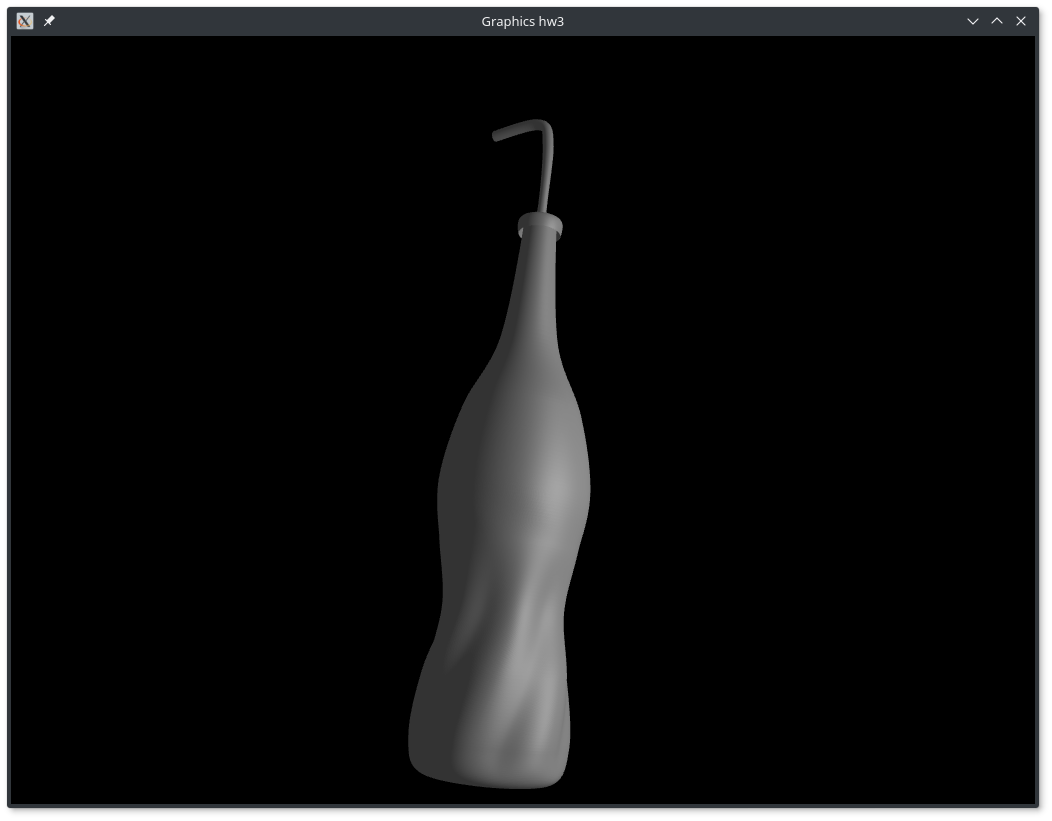
\includegraphics[width=0.75\linewidth]{coke.png}
  \end{figure}
\item
  Homework 2에서 구현한 \verb|control.cpp|의 기능들을 그대로 사용하여, 모델을 translate, rotate, zoom 등 할 수 있도록 하였다. 조작법은 앞의 Controls에 설명되어 있다.
\item
  \verb|sample.txt|에 체스 나이트 말의 모델을 간단하게 구성하였다. 렌더링 결과는 아래와 같다.
  \begin{figure}[H]
    \centering
    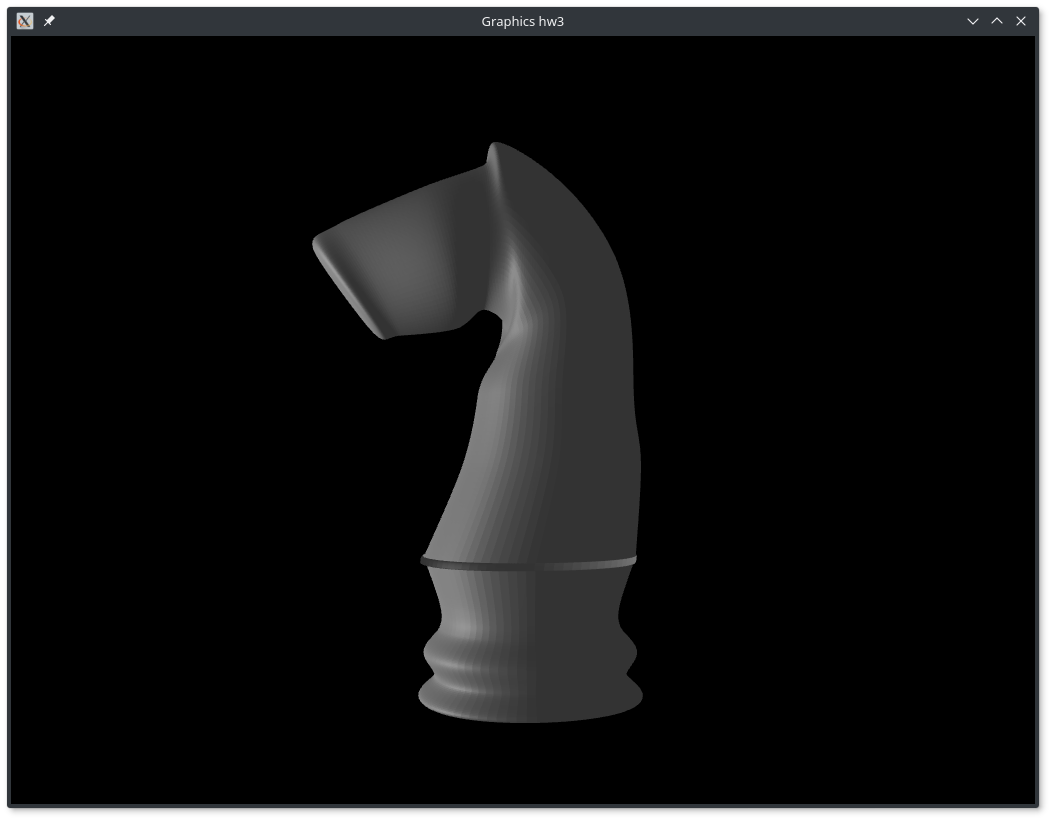
\includegraphics[width=0.75\linewidth]{knight.png}
  \end{figure}
\end{enumerate}
\end{document}
